\chapter{Android Usability Study}
\section{Einleitung}
Bei dem Projekt BestShift hat die Android Applikation eine hohe Priorität, weil diese die Daten sammelt, dem Nutzer möglichst in Echtzeit darstellt und sie außerdem auf den Server lädt um Sie dem Nutzer für eine weitere Analyse verfügbar zu machen. 
Daher ist die Android App, neben dem Car-PC, die zentrale Schnittstelle für die Daten die gesammelt werden. 

\section{Design-Umsetzung}
Das Design ist als Tab-Implementierung umgesetzt worden, was den Fahrer bei der Fahrt möglichst wenig ablenken wird, weil er um zu den unterschiedlichen Funktionen zu gelangen keinen kleinen Knopf erwischen muss, sondern den kompletten Bildschirm seines Smartphones verwenden kann. Innerhalb der einzelnen Views und Activities setzt dann jeder der App-Beteiligten seine eigenen Designs um. 

Diese Umsetzung mittels der Tab-Implementierung sieht bisher so aus.
\newpage
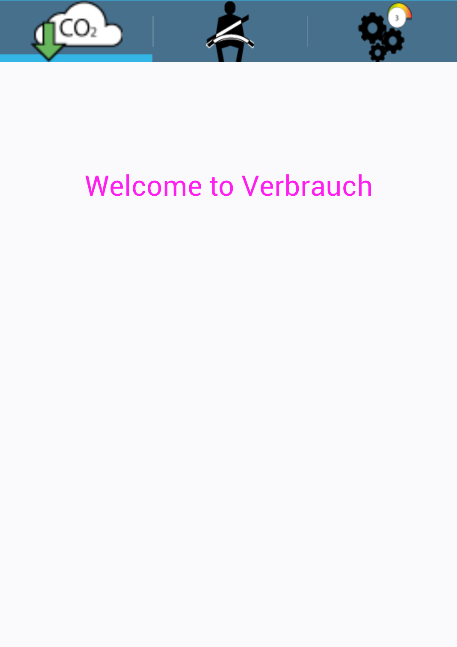
\includegraphics[scale=0.4]{images/Verbrauch.png}
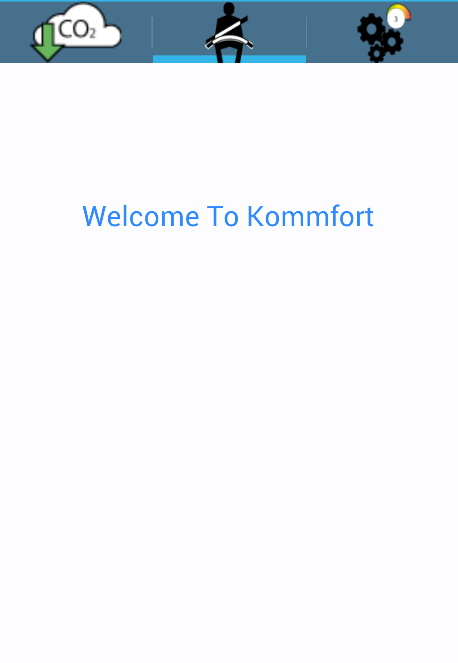
\includegraphics[scale=0.4]{images/Komfort.png}
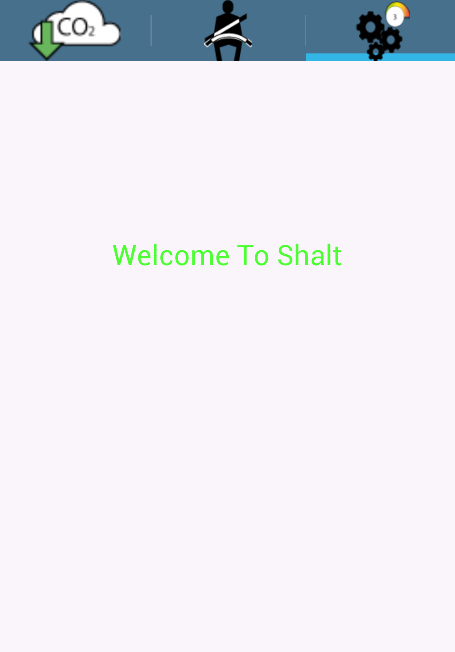
\includegraphics[scale=0.4]{images/Schalt.png}